\section{Implementation of the Safety Annex}
\label{sec:impl}
Important features were considered before the implementation of the safety annex; these we addressed one by one and will outline below. 

\textbf{Shared model} As described in Section~\ref{sec:concepts}, an AADL~\cite{AADL_Standard} model describes a system in terms of a hierarchy of components and their interconnections, where each component can either represent a logical entity (e.g., application software functions, data) or a physical entity (e.g., buses, processors). AADL is used to specify and analyze real-time embedded systems. It includes specifications specific to hardware, software, and system component abstractions. The language definition is sufficiently rigorous to support formal analysis tools that allow for early phase error/fault detection~\cite{FeilerModelBasedEngineering2012}. 

\begin{figure}[h!]
	%\vspace{-0.1in}
	\begin{center}
	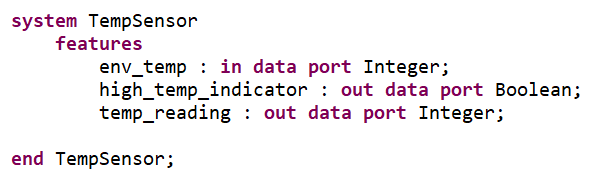
\includegraphics[width=.8\textwidth]{images/aadlComponent.png}
	\caption{An AADL Component Type Definition}
	\label{fig:aadlComponent}
	%\vspace{-0.2in}
	%\vspace{-0.1in}
	\end{center}
\end{figure}

Central to an AADL model are component \emph{type} and \emph{implementation} declarations. Figure~\ref{fig:aadlComponent} shows an example of a simple sensor component type defined in AADL. The component has an environmental temperature as input and two outputs: a high temperature indication and a temperature reading. In the type declaration, you define the category (\texttt{system} in this example) and features such as inputs and outputs; the implementation contains definitions of the internal structure of the component, e.g., internal constituents and their interactions. Figure~\ref{fig:aadlComponent} shows a component {\em type}. 

\begin{figure}[h!]
	%\vspace{-0.1in}
	\begin{center}
	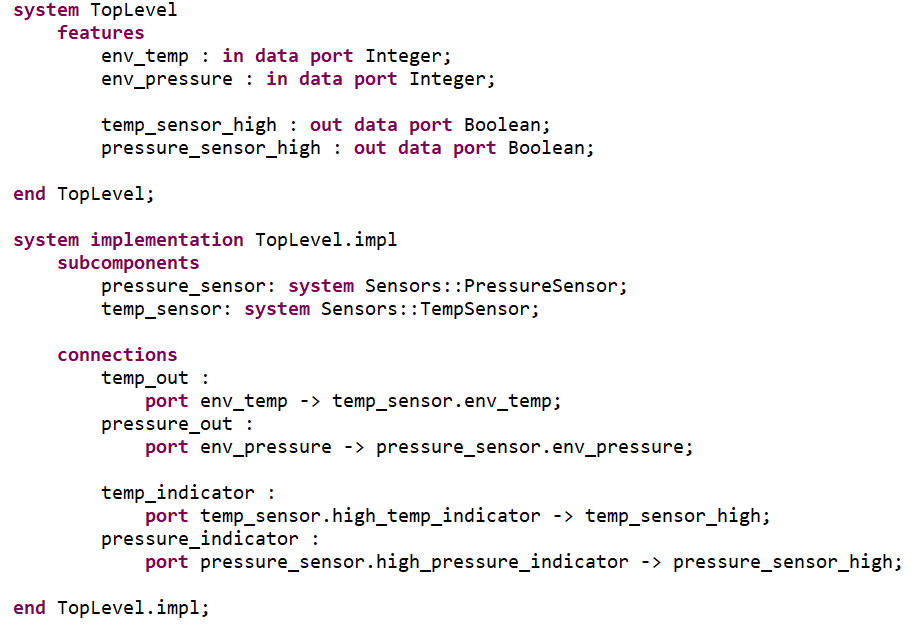
\includegraphics[width=1.0\textwidth]{images/aadlImplementation.png}
	\caption{An AADL Component Implementation Definition}
	\label{fig:aadlImplementation}
	%\vspace{-0.2in}
	%\vspace{-0.1in}
	\end{center}
\end{figure}

The implementation containing the sensor component type is shown in Figure~\ref{fig:aadlImplementation}. The system contains a type of its own (top of figure: \texttt{system TopLevel}) which holds any environmental inputs or subcomponent outputs. The implementation defines the subcomponents of the system and their connections (bottom half of figure). 

Since AADL supports model-based system development and the language definition is sufficiently rigorous to support formal analysis tools that allow for early phase error/fault detection~\cite{FeilerModelBasedEngineering2012}, this language was chosen for this research. 

\textbf{Behavioral analysis} As described in Section~\ref{subsec:mbsa}, {\em nominal model analysis} is a part of the MBSA process. The nominal model consists of the system model architectural design as well as behavioral contracts for each component and requirement specifications. The verification at the nominal level consists of showing that the model satisfies the specified requirements in the absence of faults. 

The Assume-Guarantee Reasoning Environment (AGREE)~\cite{cofer2012compositional} is a language annex for AADL that provides a mechanism for the specification of component requirements in formal logic and utilizes a model checker to provide proofs regarding these specifications as described in Section~\ref{sec:concepts}. 

\begin{figure}[h!]
	%\vspace{-0.1in}
	\begin{center}
	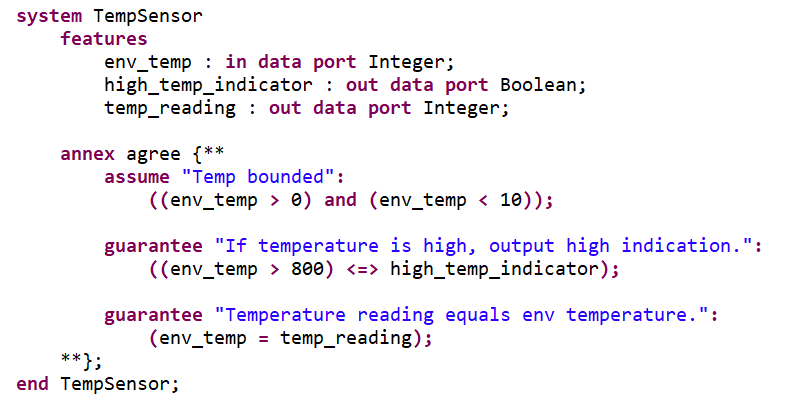
\includegraphics[width=1.0\textwidth]{images/agreeContract2.png}
	\caption{The AGREE Contract for an AADL Component Type}
	\label{fig:agreeContract}
	%\vspace{-0.2in}
	%\vspace{-0.1in}
	\end{center}
\end{figure}

An example of an AGREE contract is shown in Figure~\ref{fig:agreeContract} and is placed in the context of the AADL temperature sensor component shown in Figure~\ref{fig:aadlComponent}.  An AGREE contract consists of {\em assumptions} on the inputs of AADL components that constrain what the component sees from the environment and {\em guarantees} on the outputs that constrain how the component behaves given its environment. In this example, the assumption restricts the environmental temperature to be within a range of values; the guarantee defines the behavior of the component given the environment. 

Since our desire was to facilitate {\em behavioral error propagation}, AGREE was a suitable and obvious choice for the nominal verification tooling. 

\textbf{Model checker} Through AGREE, the nominal model is translated into the dataflow programming language Lustre~\cite{Halbwachs91:IEEE} which is then used as input to the JKind model checker~\cite{2017arXiv171201222G}. JKind uses a series of backend SMT-solvers to generate proofs of the top level AGREE properties specified in the model. When there exists a trace such that a property is invalid, JKind provides a {\em counterexample} showing the state of the system in which the property is violated. An example of this is shown in Figure~\ref{fig:coex}. 

\begin{figure}[h!]
	%\vspace{-0.1in}
	\begin{center}
	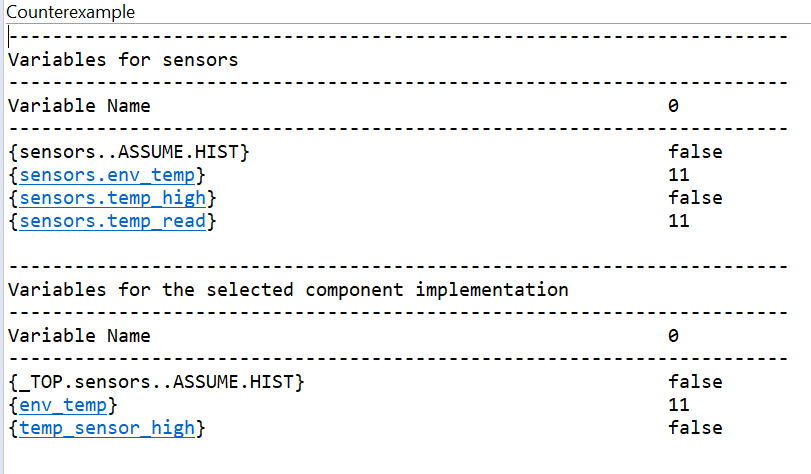
\includegraphics[width=1.0\textwidth]{images/coex.png}
	\caption{A Counterexample to an Invalid Property}
	\label{fig:coex}
	%\vspace{-0.2in}
	%\vspace{-0.1in}
	\end{center}
\end{figure}

The model checker takes an adversarial role in the proof process by trying to find paths such that the proof is violated. If none exist, then the results are valid. This adversarial role is exactly what we wished to harness for this kind of analysis. If we allow faults to be active, but leave them unconstrained, this allows the model checker to determine if certain faults could violate a proof. These counterexamples could then contain fault information. 

\textbf{Behavioral error propagations} Given that AGREE guarantees define the {\em output} behavior of components, any connected component's assumptions rely on those guarantees. If an assumption is violated, the guarantee may not hold. By associating a fault with the output of a component, this fault -- when active -- may violate assumptions and guarantees along the signal flow within a system. This was our goal; we wished to view the behavioral propagation of an active fault. 

\subsection{Implementation Architecture}
\label{sec:implArchitecture}
The safety annex is written in Java as a plug-in for the OSATE AADL toolset, which is built on Eclipse.  It is not designed as a stand-alone extension of the language, but works with behavioral contracts specified using the AGREE annex for AADL~\cite{NFM2012:CoGaMiWhLaLu}. 
The architecture of the Safety Annex is shown in Figure~\ref{fig:plugin-arch}.

\begin{figure}[h]
	\begin{center}
		%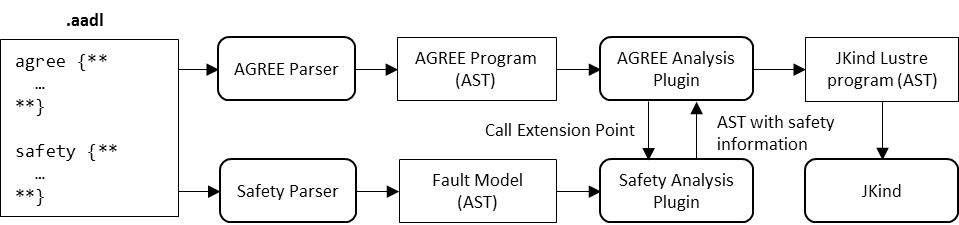
\includegraphics[trim=0 400 430 0,clip,width=0.85\textwidth]{images/arch.png}
		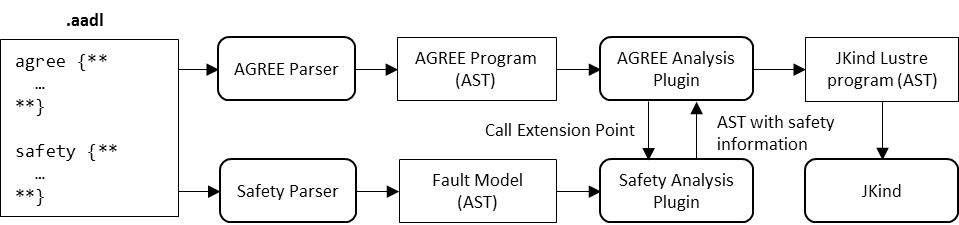
\includegraphics[width=\textwidth]{images/arch.png}
	\end{center}
	%\vspace{-0.2in}
	\caption{Safety Annex Plug-in Architecture}
	\label{fig:plugin-arch}
	%\vspace{-0.2in}
\end{figure}

The safety language extension resides in an annex of AADL and the faults defined therein are translated into an abstract syntax tree and inserted into the AGREE program. The AGREE program contains the building blocks for the translation into Lustre which is the program directly analyzed by JKind.  

When performing fault analysis, the fault definitions defined in the safety annex extend the AGREE contracts to allow faults to modify the behavior of component outputs. The temperature sensor subcomponent shown in Figure~\ref{fig:agreeContract} encoded into Lustre is shown in Figure~\ref{fig:lustreTempNode}\footnote{The Lustre code is slightly simplified for readability.}.

\begin{figure}[h]
	\begin{center}
		%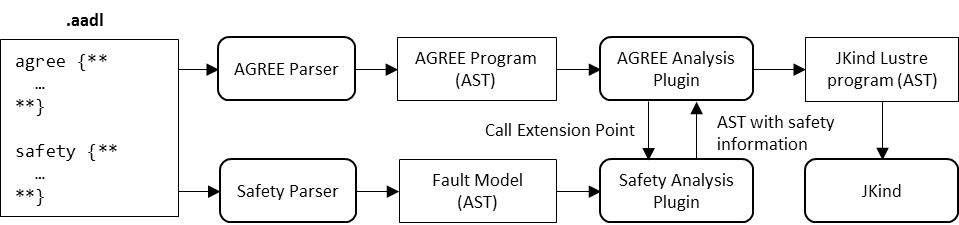
\includegraphics[trim=0 400 430 0,clip,width=0.85\textwidth]{images/arch.png}
		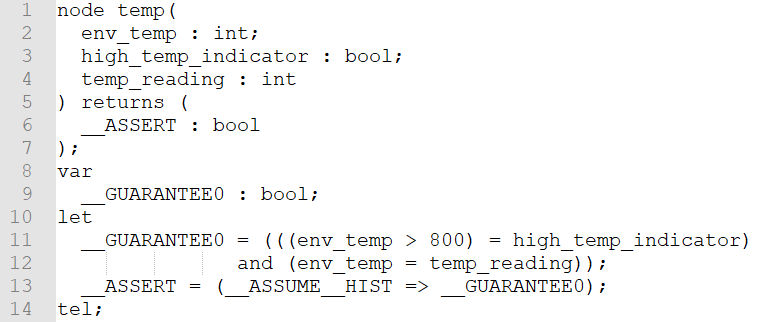
\includegraphics[width=0.8\textwidth]{images/lustreTempNode.png}
	\end{center}
	%\vspace{-0.2in}
	\caption{Temperature Component in Lustre}
	\label{fig:lustreTempNode}
	%\vspace{-0.2in}
\end{figure}

The inputs and outputs (lines 2-4) correspond directly to the AADL inputs and outputs of the component; likewise, the guarantee (\texttt{\_\_GUARANTEE0}) corresponds to the guarantee on the outputs. The \texttt{\_\_ASSERT} statement on line 13 just states that as long as the assumptions hold, the guarantee is implied. 

From the perspective of fault analysis, we want to insert a fault on the output of the component. This fault may or may not be active -- it is up to the model checker. To this end, we specify three variables per potentially faulty output: \texttt{fault\_nominal}, \texttt{fault\_trigger}, and \texttt{fail\_val}. If the trigger is true, then output failure value, else output nominal value. This can be seen in Figure~\ref{fig:lustreTempNodeFault}: the new variables are assigned as inputs (lines 4-6) and the assert statement in line 20 shows the triggering behavior.

\begin{figure}[h]
	\begin{center}
		%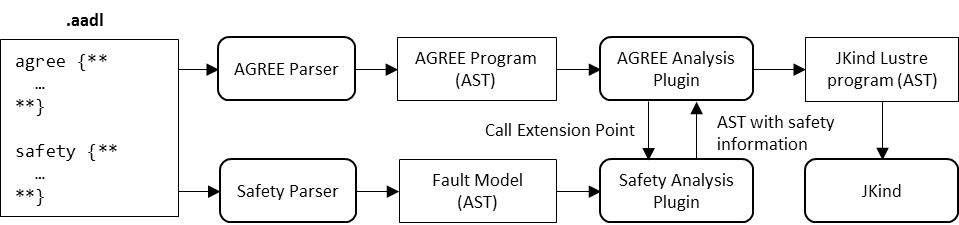
\includegraphics[trim=0 400 430 0,clip,width=0.85\textwidth]{images/arch.png}
		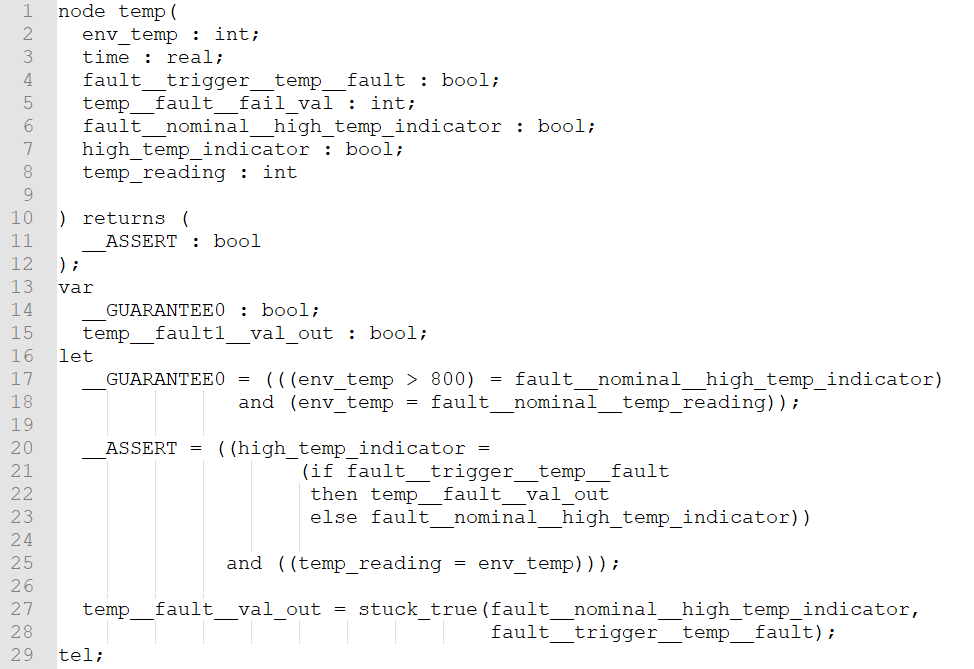
\includegraphics[width=0.8\textwidth]{images/lustreTempNodeFault.png}
	\end{center}
	%\vspace{-0.2in}
	\caption{Temperature Component with Fault in Lustre}
	\label{fig:lustreTempNodeFault}
	%\vspace{-0.2in}
\end{figure}

This allows for the possibility of active faults, but when the faults are inactive, the nominal value is simply passed through. Line 27 of Figure~\ref{fig:lustreTempNodeFault} shows a call to what we call a {\em fault node}; this is the code that specifies the behavior of an active fault. The fault node \texttt{stuck\_true} is shown in Figure~\ref{fig:lustreFaultNode}. The behavior of an active fault is to output {\em true}. The \texttt{trigger} input to the fault node corresponds directly with the trigger defined in the temperature node of Figure~\ref{fig:lustreTempNodeFault} on line 4. 

\begin{figure}[h]
	\begin{center}
		%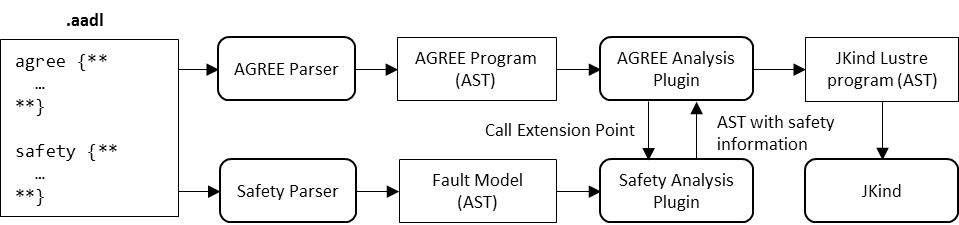
\includegraphics[trim=0 400 430 0,clip,width=0.85\textwidth]{images/arch.png}
		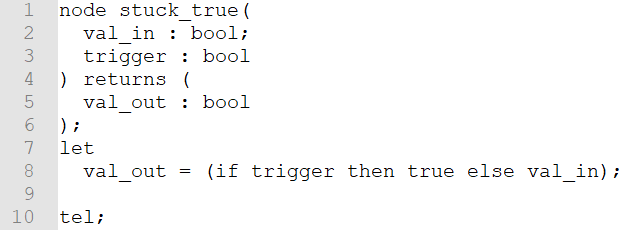
\includegraphics[width=0.8\textwidth]{images/lustreFaultNode.png}
	\end{center}
	%\vspace{-0.2in}
	\caption{A Fault Node in Lustre}
	\label{fig:lustreFaultNode}
	%\vspace{-0.2in}
\end{figure}

\begin{comment}
There are two different types of fault analysis that can be performed on a fault model. The Safety Annex plugin intercepts the AGREE program and add fault model information to the model depending on which form of fault analysis is being run.

\textbf{Verification in the Presence of Faults}: This analysis returns one counterexample when fault activation per the fault hypothesis can cause violation of a property. The augmentation from Safety Annex to the AGREE program includes traceability information so that when counterexamples are displayed to users, the active faults for each component are visualized.

\textbf{Generate Minimal Cut Sets}: This analysis collects all minimal set of fault combinations that can cause violation of a property. As described in Chapter~\ref{chap:mcsGen}, the first step of MinCutSet generation is to collect the minimal IVCs for each property. Given the compositional nature of the verification, each level of the system is extended in a slightly different way. The leaf nodes of a system contribute only constrained faults to the \aivcalg algorithm as shown in Figure~\ref{fig:ivcElements1}. 

\begin{figure}[h!]
	\hspace*{-2cm}
	\vspace{-0.1in} 
	\begin{center}
		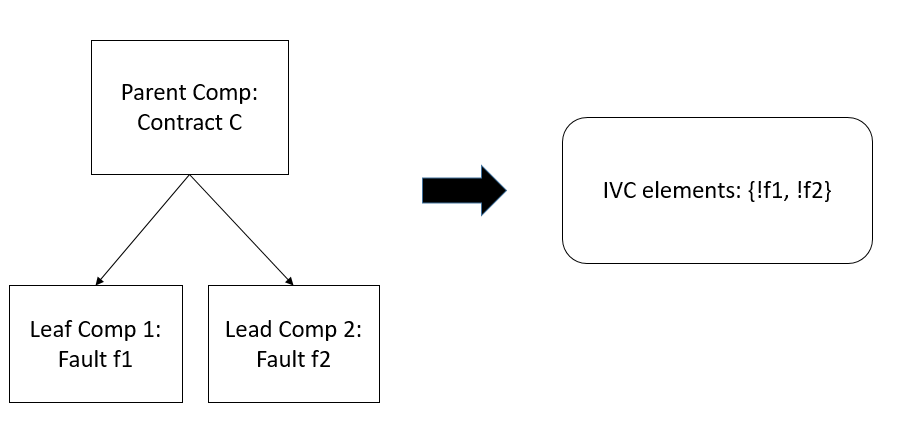
\includegraphics[scale=0.5]{images/ivcElements1.png}
	\caption{IVC Elements used for Consideration in a Leaf Layer of a System}
		\label{fig:ivcElements1}
	\end{center}
\end{figure}

In the non-leaf layers of the program, both contracts and constrained faults are considered as shown in Figure~\ref{fig:ivcElements2}. The reason for this is that the contracts are used to prove the properties at the next highest level and are necessary for the verification of the properties. 

\begin{figure}[h!]
	\hspace*{-2cm}
	\vspace{-0.1in} 
	\begin{center}
		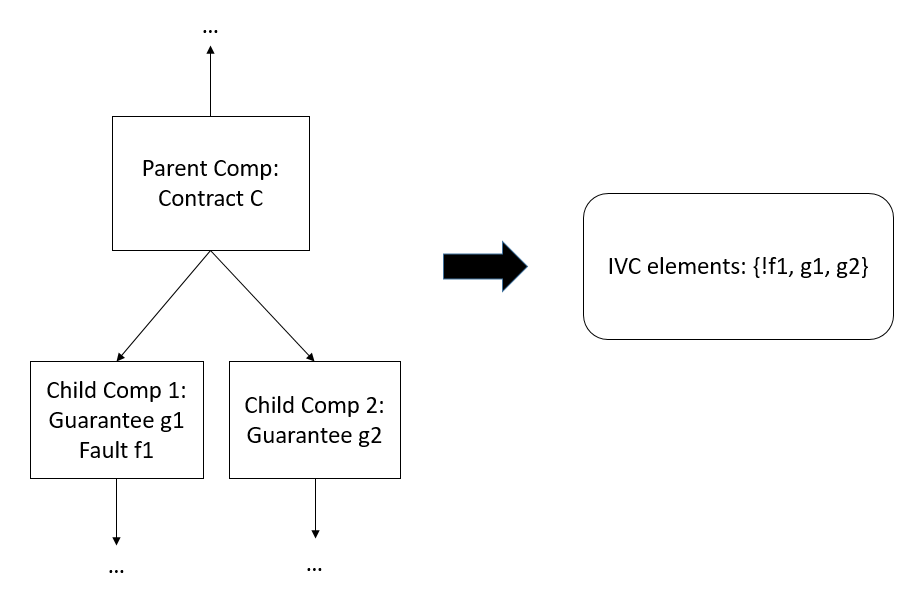
\includegraphics[scale=0.5]{images/ivcElements2.png}
	\caption{IVC Elements used for Consideration in a Middle Layer of a System}
		\label{fig:ivcElements2}
	\end{center}
\end{figure}

The \aivcalg algorithm returns the minimal set of these elements necessary to prove the properties. This equates to any contracts or inactive faults that must be present in order for the verification of properties in the model. From here, we transform all MIVCs into minimal cut sets.

\end{comment}